\documentclass{beamer} %
%\usetheme{CambridgeUS}
\usepackage[latin1]{inputenc}
%\usefonttheme{professionalfonts}
\usepackage{times}
\usepackage{tikz}
\usepackage{amsmath}
\usepackage{verbatim}
\usetikzlibrary{positioning,shapes,shadows,arrows}

%style
\tikzstyle{every picture}+=[remember picture]
\definecolor{azul}{RGB}{29,186,222}
\definecolor{morado}{RGB}{161,29,222}
\definecolor{marron}{RGB}{223,66,30}
\definecolor{verde}{RGB}{90,222,29}

%node style
\tikzstyle{frame}=[rectangle, rounded corners, text centered, anchor=north, text width=2.5cm, text=black, draw=black!80!azul!20, top color=white, bottom color=azul]
\tikzstyle{label}=[]

%arrow styles
\tikzstyle{fixed}=[->, black!50, thick]
\tikzstyle{estimation}=[->, morado, thick, dashed]
\tikzstyle{difference}=[->, marron, thick, dotted]
\tikzstyle{source}=[->, verde, thick]


%metadata
\title{Integration of multiple localization systems into TF}
\author{Pablo Urcola \\ \texttt{urcola@unizar.es}}
\institute{Universidad de Zaragoza, Spain}
\date{2015 European Robotics Forum. ROS Community Workshop}

\begin{document}

\begin{frame}
\titlepage
\end{frame}

\begin{frame}
\frametitle{TF tree}
\vspace{3cm}
%\begin{figure}[*ht]
\begin{center}
\begin{tikzpicture}[node distance=1.0cm, auto, overlay]
%nodes
	\node<1-> [frame]                                (robot) {robot};
	\node<2-> [frame, above=of robot]                (odom) {odom};
	\node<3-> [frame, above=of odom]                 (map) {map};
	\node<4-> [label, right=of odom, morado] (amcl) {AMCL};
	\node<5-> [label, above=of odom, marron, xshift=-1.0cm, yshift=-0.75cm] (mapcorrection) {Correction};
	\node<6-> [frame, above=of map]                  (gps) {gps};
	\node<7-> [label, left=of odom, morado, xshift=-0.9cm]  (ekf) {EKF};
	\node<7-> [frame, below=of robot]                (antenna) {antenna};	
	\node<8,9> [label, above=of map, marron, xshift=-1.0cm, yshift=-0.75cm] (gpscorrection) {Correction};

%edges		
	\path<2->  (odom)  edge [estimation, out=270, in=90]  node[auto, swap] {Odometry}              (robot);
	\path<4->  (map)   edge [estimation, out=0, in=0]                                              (robot);
	\path<5->  (map)   edge [difference, out=270, in=90]                                           (odom);
	\path<5->  (amcl)  edge [source, out=180, in=0]                                                (mapcorrection);
	\path<7->  (robot) edge [fixed, out=270, in=90]       node[auto]       {Fixed}                 (antenna);
	\path<7->  (gps)   edge [estimation, out=180, in=180]                                          (antenna);
	\path<8->  (gps)   edge [difference, out=270, in=90]                                                (map);
	\path<8,9>   (ekf)   edge [source, out=0, in=180]       										 (gpscorrection);
	\path<8,9>   (amcl)  edge [source, out=180, in=0]       										 (gpscorrection);	
	\path<10>  (gps)  edge [fixed, out=270, in=90]       node[auto]      {Fixed} (map);
	\path<10>  (ekf)  edge [source, out=0, in=180]       (mapcorrection);
\end{tikzpicture}
\end{center}
%\end{figure}
\vspace{2cm}
\uncover<9>{Problem: Where is the robot in the map frame?}

\uncover<10>{A new node manages the tf publication.}
\end{frame}

\begin{frame}
\frametitle{Conclusions}
\begin{itemize}
	\item Multiple estimation of robot position cannot be directly introduced into TF
	\item Using the map-odom correction technique, fixed frames become not-fixed
	\item Disabling tf publishers is required to have only one correction point
\end{itemize}
\end{frame}

\end{document}